\documentclass[11pt,letterpaper]{article}
\usepackage[margin=0.85in]{geometry}
\usepackage[T1]{fontenc}
\usepackage[utf8]{inputenc}
\usepackage{lmodern,microtype}
\DisableLigatures{encoding=T1,family=lmtt}
\usepackage{amsmath,amssymb}
\usepackage{booktabs,tabularx,array,longtable}
\usepackage{xcolor,tikz}
\usetikzlibrary{arrows.meta,positioning}
\usepackage{enumitem,listings,fancyhdr,hyperref}
\definecolor{navy}{HTML}{173553}
\definecolor{teal}{HTML}{167D8D}
\definecolor{pale}{HTML}{F1F6FA}
\hypersetup{colorlinks=true,linkcolor=navy,citecolor=teal,urlcolor=teal,
 pdftitle={Can a Computer Hear a Drone? An Accessible Research Paper on Classical Acoustic Detection},
 pdfauthor={QubitSky Project}}
\setlength{\parindent}{0pt}
\setlength{\parskip}{5pt}
\setlength{\headheight}{14pt}
\setlist{itemsep=3pt,topsep=4pt}
\pagestyle{fancy}
\fancyhf{}
\lhead{\small QubitSky | An Accessible Research Paper}
\rhead{\small Classical Models A--D}
\cfoot{\small\thepage}
\newcolumntype{Y}{>{\raggedright\arraybackslash}X}
\newcommand{\code}[1]{\texttt{\detokenize{#1}}}
\newcommand{\R}{\mathbb{R}}
\newcommand{\plain}[1]{\par\smallskip\noindent\textbf{In everyday language.} #1\par\smallskip}
\lstset{basicstyle=\ttfamily\footnotesize,breaklines=true,columns=fullflexible,
 keepspaces=true,showstringspaces=false,backgroundcolor=\color{pale},
 frame=single,rulecolor=\color{navy!20}}

\title{\textcolor{navy}{\textbf{Can a Computer Hear a Drone?}}\\[7pt]
 \Large A Classical Machine-Learning Approach to\\Acoustic Drone Detection Under Noise\\[7pt]
 \large An Accessible Research Paper and Experimental Proposal}
\author{QubitSky Project}
\date{October 7, 2026}
\begin{document}
\maketitle
\thispagestyle{fancy}

\begin{abstract}
A microphone records pressure changes, not a label saying ``drone.'' The
research problem is to learn which patterns in those measurements distinguish
drones from confusing background sounds, including when recordings are noisy
and independent training examples are scarce. This paper explains a four-model
classical approach from first principles: an RBF support vector machine (A),
a small multilayer perceptron (B), a larger multilayer perceptron (C), and a
convolutional neural network (D). It motivates their different roles, derives
the main preprocessing and evaluation equations, identifies public data
sources, and proposes a comparison that keeps source recordings separate across
training, validation, and test sets. The presentation assumes no prior
machine-learning knowledge while retaining an academic problem statement,
research questions, methods, experimental design, limitations, and references.
No new training or empirical performance measurements are reported. Numerical
examples are explicitly instructional. The contribution is an explained,
testable study design, not a claim that one model or quantum method has won.
\end{abstract}

\textbf{Keywords:} acoustic drone detection; classical baselines; limited
training data; environmental noise; source-group separation; reproducibility.

\textbf{How to read this paper.} Begin with the plain-language paragraphs and
figures. Each equation is followed by the meaning of its symbols. Sections
\ref{sec:fourmodels}--\ref{sec:modeld} explain the models individually;
Section~\ref{sec:metrics} gives a worked evaluation example. Appendix~\ref{sec:glossary}
defines the recurring terms. This uses the structure of a research paper; it is
not presented as an awarded dissertation or a completed experimental study.

\section{Introduction: the problem before the models}
\label{sec:intro}
Imagine an outdoor microphone recording a mixture of a flying drone, wind,
traffic, and insects. A useful detector should raise an alert when drone sound
is present and avoid raising one merely because a different sound resembles
it. The microphone does not separate those sources for us. It measures their
combined effect at its location.

This project studies \emph{binary classification}: assigning one of two labels
to an audio example. Here, 1 means drone and 0 means non-drone. The current
scope is presence classification; it does not establish the drone's identity,
position, distance, intent, or flight path. Those would require different
labels, methods, and evaluations.

Three difficulties motivate the study. First, different physical sources can
produce similar measured patterns. Second, additional noise can obscure a cue
that was clear in a quiet recording. Third, collecting many genuinely
independent flights, locations, and conditions is different from cutting one
recording into many small pieces. A model can appear successful by remembering
the recording environment instead of learning a transferable drone cue.

\plain{We want a detector that recognizes a new drone recording, not one that
merely recognizes the background of a recording it has already heard.}

\subsection{Why begin with classical models?}
``Classical'' means conventional computation, as opposed to the quantum-kernel
methods considered elsewhere in the project. It does not mean obsolete or
necessarily weak. A meaningful quantum comparison needs credible classical
alternatives on the same problem. Otherwise, a reported difference could arise
from input features, tuning effort, or data leakage rather than the quantum
method itself.

Using four baselines also makes the classical study informative on its own.
It separates the effect of a kernel classifier, a small neural network, a
larger neural network, and a richer audio representation. The method that is
best for a compact, low-data experiment need not be best for an application
with more data and compute.

\subsection{Research questions and falsifiable expectations}
\begin{enumerate}[label=\textbf{RQ\arabic*.}]
 \item How do A--D respond when independent training-recording counts decrease?
 \item How do drone recall and false alarms change as added noise increases?
 \item Does additional neural capacity help when the input features stay fixed?
 \item Does preserving a time-frequency representation help enough to justify
 its additional computation and input information?
 \item Under exactly matched compact inputs and data budgets, does a quantum
 model improve on the classical alternatives?
\end{enumerate}
Plausible expectations are that noise will make detection harder and that
additional capacity may help when sufficient information and data are available.
Neither is assumed to hold monotonically for every fitted model or finite
test set. A result in which B matches C, or A exceeds D, would be scientifically
useful rather than a failure of the experiment.

\section{Background: the minimum vocabulary}
\subsection{Sound, samples, windows, and features}
A digital waveform is a sequence of numbers describing a microphone signal
over time. The \emph{sample rate} is how many measurements are stored each
second. At 16 kHz, one second contains 16,000 numbers. A \emph{window} is a
short contiguous portion of that waveform. It is a unit of processing, not
automatically an independent recording.

A \emph{feature} is a number computed from the audio to summarize something
about it. A small set of features is like a short description of a much longer
recording. Compression makes learning and comparison manageable, but can throw
away the very distinction the classifier needs. A classifier cannot recover
information it never receives.

\subsection{Learning, inference, and overfitting}
During \emph{training}, an algorithm adjusts model parameters using labeled
examples. During \emph{inference}, those parameters stay fixed while the model
scores a new example. A \emph{hyperparameter}, such as the number of hidden
units, is a setting chosen outside the fitting procedure. Searching many such
settings is still part of model development and must not use the test labels.

\emph{Overfitting} occurs when fitting the available examples does not translate
into good performance on new independent examples. \emph{Underfitting} means
the model or representation is too restrictive to capture useful patterns in
the task. More parameters can change this tradeoff, but parameter count alone
does not predict which model will generalize.

\subsection{The three data partitions}
Training, validation, and test data have different jobs:
\begin{center}
\begin{tabularx}{\linewidth}{@{}lYY@{}}
\toprule
Partition & Purpose & Everyday analogy \\
\midrule
Training & Fit weights and preprocessing & Practice material used to learn \\
Validation & Choose settings and checkpoints & A practice exam used to revise the approach \\
Test & Evaluate the frozen procedure & A final exam that does not guide revisions \\
\bottomrule
\end{tabularx}
\end{center}
The analogy has a strict consequence: repeatedly changing the model after
looking at its test score turns that test into development data. A new,
untouched evaluation set would then be needed for an unbiased final assessment.

\section{Related work and the role of this paper}
Support vector networks formalize a margin-based approach to
classification~\cite{svmoriginal}. The present implementation uses an RBF SVM
through scikit-learn~\cite{svc}. Small and larger feed-forward networks are
implemented with \code{MLPClassifier}~\cite{mlp}; the CNN uses convolutional
parameter sharing~\cite{convbook}, dropout~\cite{dropout}, and Adam
optimization~\cite{adam}.

The data references are equally important. DDL supplies drone-audio
resources~\cite{ddl}; ESC-50 and UrbanSound8K supply environmental and urban
sound collections~\cite{esc50,urbansound}; NASA supplies external flyover
recordings~\cite{nasa}. Svanstr\"om and ITU ARIS resources are also relevant
to the teammate's experiment~\cite{svanstrom,ituaris}.

This paper does not propose a new classifier architecture or a new benchmark
record. Its purpose is to explain why these established methods form a useful
comparison and how to keep that comparison interpretable. Code availability,
a successful software test, and convincing detection accuracy are three
different kinds of evidence.

\section{Problem formulation and dataset design}
\label{sec:data}
Let $x_r$ denote the waveform of source recording $r$, and let $y_r\in\{0,1\}$
be its label. The model produces a score $s_r$ and a binary decision
\begin{equation}
 \widehat{y}_r=\mathbf{1}\{s_r\geq\tau\}.
 \label{eq:decision}
\end{equation}
The symbol $\mathbf{1}$ means ``return 1 if the condition is true and 0
otherwise.'' The threshold $\tau$ is the score required for a positive
decision. Its default is zero for the SVM decision score and 0.5 for the
neural-network outputs. These are implementation choices, not universal
operating points for every deployment.

\plain{The model gives every recording a number. The threshold is the pass
mark. At or above the pass mark, the answer is ``drone''; below it, the answer
is ``not a drone.'' Moving the pass mark changes how cautious the detector is.}

\subsection{Which datasets answer which part of the question?}
\begin{center}
\small
\begin{tabularx}{\linewidth}{@{}>{\raggedright\arraybackslash}p{3.2cm}YY@{}}
\toprule
Source & Intended contribution & What must remain separate \\
\midrule
DDL~\cite{ddl} & Real drone recordings & Original sessions and sequential fragments \\
ESC-50~\cite{esc50} & Relevant non-drone sounds and additive noise & Source IDs and confuser/noise roles \\
UrbanSound8K~\cite{urbansound} & Urban and mechanical confusers/noise & Source IDs and published fold metadata \\
NASA Small UAS~\cite{nasa} & External-domain flyover audio & All training and validation decisions \\
Svanstr\"om; ITU ARIS~\cite{svanstrom,ituaris} & Sources referenced by the teammate protocol & Their exact release and grouping rules \\
\bottomrule
\end{tabularx}
\end{center}
The project downloader selects DDL's real archive rather than its synthesized
archive. The documented naming scheme includes drone and no-drone codes, but
the repository's inventory notes report no no-drone-coded files in the
inspected real archive. We must therefore verify label availability, rather
than assume the dataset name implies a ready-made balanced binary task.

ESC-50 selections include aircraft-like, weather, animal, alarm, and transient
sounds. UrbanSound8K selections include engine idling, sirens, car horns,
drilling, jackhammers, gun shots, and street music. These are useful negative
examples because the task is to reject plausible confusers, not merely to
distinguish a drone from an unrelated quiet recording. The project-specific
binary task is not the original multiclass benchmark of either corpus.

NASA is reserved for external evaluation: testing transfer to a different
collection process. If reliable labels are missing, predictions can be
summarized, but accuracy and F1 cannot be computed honestly. If an external
subset contains only positive examples, it also cannot establish how well the
detector rejects negative examples.

\subsection{Independence is more important than the file count}
Suppose one minute of audio is divided into sixty one-second files. These are
sixty windows, but they may still share one flight, location, microphone, and
weather condition. Randomly assigning the files to training and test allows
related information onto both sides of the split.

\plain{Cutting one photograph into sixty pieces does not create sixty
independent photographs. Cutting audio into windows has the same problem.}

Every related file must retain a source-group identifier. Split those groups
first, then derive windows and noisy versions. The ITU ARIS release explicitly
includes overlapping segments and interval mappings; preserve its grouping
protocol~\cite{ituaris}. Keep ESC-50 and UrbanSound8K source identifiers and
resolve overlaps between them when they refer to the same Freesound recording.
An additive noise donor must not carry held-out source audio into training.

\section{Turning recordings into model inputs}
\label{sec:processing}
\begin{figure}[htbp]
\centering
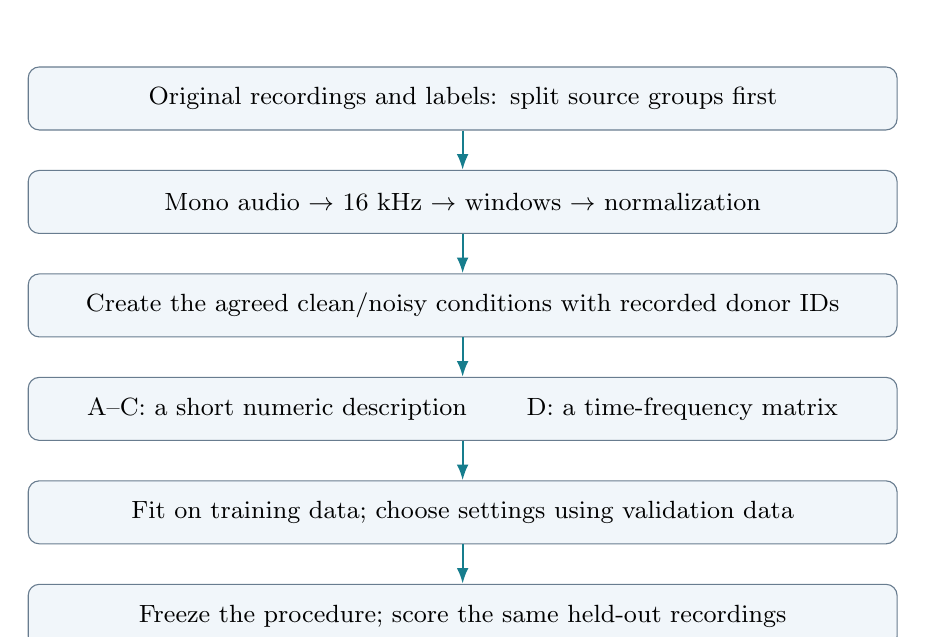
\begin{tikzpicture}[
 node distance=5mm,
 b/.style={draw=navy!65,fill=pale,rounded corners,align=center,
 text width=10.8cm,minimum height=8mm,font=\small},
 a/.style={-{Latex[length=2mm]},thick,draw=teal}]
 \node[b] (s) {Original recordings and labels: split source groups first};
 \node[b,below=of s] (w) {Mono audio $\rightarrow$ 16 kHz $\rightarrow$ windows $\rightarrow$ normalization};
 \node[b,below=of w] (n) {Create the agreed clean/noisy conditions with recorded donor IDs};
 \node[b,below=of n] (f) {A--C: a short numeric description \qquad D: a time-frequency matrix};
 \node[b,below=of f] (t) {Fit on training data; choose settings using validation data};
 \node[b,below=of t] (e) {Freeze the procedure; score the same held-out recordings};
 \draw[a] (s)--(w); \draw[a] (w)--(n); \draw[a] (n)--(f);
 \draw[a] (f)--(t); \draw[a] (t)--(e);
\end{tikzpicture}
\caption{The order of operations is part of the method. Feature fitting and
model selection are not allowed to learn from the test set.}
\end{figure}

\subsection{A common waveform format}
Recordings are converted to mono and resampled to 16 kHz so that a sample
position has a consistent time meaning. The baseline uses non-overlapping
windows; a final incomplete window is padded with zeros. One-second windows
contain 16,000 samples; three-second windows contain 48,000. A shorter window
offers less context, while a longer window can mix a brief event with more
background. This is a protocol choice to validate, not a rule that longer is
always better.

Each window is peak-normalized by dividing by its largest absolute value,
with a small denominator floor to handle zero-valued audio. Consequently, the
method deliberately reduces dependence on absolute recording amplitude.
That may reduce sensitivity to recording gain, but also removes amplitude
information that could be useful. Resampling and normalization do not make
different recording environments identical.

\subsection{Noise and the meaning of SNR}
\plain{Signal-to-noise ratio (SNR) says how strong the recording we care about
is compared with the noise we deliberately add on top. A large positive number
means the added noise is faint. Zero means the two are equally strong. A
negative number means the added noise is stronger than the recording.}

The \emph{root mean square} (RMS) measures the waveform's effective amplitude:
\begin{equation}
 R(x)=\sqrt{\frac{1}{N}\sum_{i=1}^{N}x[i]^2}.
\end{equation}
Here $N$ is the number of samples. For background $n$ and desired SNR $s$,
\begin{equation}
 x_s=x+\frac{R(x)}{R(n)}10^{-s/20}n.
 \label{eq:noise}
\end{equation}
The multiplier adjusts the added noise to the requested strength. The code
uses floating-point mixtures without clipping after mixing. SNR compares the
original target recording to the \emph{added} noise; a field recording can
already contain background sound, so ``clean'' means no additional mixture,
not a physically isolated drone.

\begin{center}
\begin{tabular}{@{}lrr@{}}
\toprule
SNR & Target-to-added-noise power ratio & Interpretation \\
\midrule
20 dB & $100:1$ & Much less added noise power \\
10 dB & $10:1$ & Less added noise power \\
5 dB & Approximately $3.16:1$ & Intermediate condition \\
0 dB & $1:1$ & Equal power \\
$-10$ dB & $1:10$ & More added noise power \\
\bottomrule
\end{tabular}
\end{center}
These ratios are definitions, not measured model performance. The shared
protocol uses clean/20/10/5/0 dB; the original baseline also supports $-10$ dB.
Use the same selected donor across SNR levels so the comparison changes noise
strength rather than donor identity. Silence has no defined target SNR; apply
one explicit exclusion/error policy, record it, and keep compared examples aligned.

\subsection{A--C: describing a sound with a few numbers}
A mel spectrogram describes energy over time in frequency bands. The mel
spacing is a frequency representation, not a drone detector. The code uses
64 bands, a 512-sample FFT, and a 160-sample hop. Its log-mel values feed the
MFCC computation~\cite{librosa}. MFCC means and standard deviations summarize
the spectral shape and how its coefficients vary during a window.

For coefficient $j$, let $c_{j,t}$ be its value at frame $t$. Then
\begin{equation}
 \mu_j=\frac{1}{T}\sum_t c_{j,t},\qquad
 \sigma_j=\sqrt{\frac{1}{T}\sum_t(c_{j,t}-\mu_j)^2}.
\end{equation}
There are 13 means and 13 standard deviations, giving 26 numbers per window.
The mean describes the average; the standard deviation describes variability.
Their ordering over time is lost. Two sequences can share the same mean and
standard deviation even when their temporal arrangements differ.

The original tabular pipeline standardizes these features, reduces them with
principal component analysis (PCA), and scales the retained coordinates into
$[0,\pi]$. Standardization prevents differently scaled coordinates from
dominating merely through their units. PCA finds directions of training-data
variation and retains $k\in\{2,4,6\}$ coordinates. Large variance does not
necessarily mean useful class information. Scaling into an angle interval
makes the representation convenient to export for quantum experiments; it does
not make the classical calculation quantum.

\plain{The waveform is the full recording. MFCC statistics are a short
description. PCA makes that description shorter still. The classifier only
gets the final description, so every compression step can matter.}

All fitted transformations must learn their statistics from the actual training
subset. The teammate's selected-feature mode is an alternative representation,
not another name for PCA. Matching the number of coordinates is insufficient
unless the values, order, and transformations also match.

\subsection{D: preserving the time-frequency matrix}
\plain{A--C are handed a short note about the sound. D is handed the whole
chart: which pitches were present at each moment. The chart holds more
information, but it is also much bigger and takes more work to learn from.}

D receives the 64-band log-mel matrix itself. A one-second window gives
$64\times101$ entries under the baseline framing. Time lies on one axis and
frequency band on the other. Although it can be displayed as a colored image,
the CNN receives numbers rather than a screenshot with axes or captions.
One mean and standard deviation, calculated from training spectrograms,
normalize the matrices. D therefore has access to structure that the compact
statistics may discard.

\section{Why four models instead of one?}
\label{sec:fourmodels}
The letters describe four complementary scientific questions:
\begin{center}
\begin{tabularx}{\linewidth}{@{}lYY@{}}
\toprule
Model & Plain-language description & Question it helps answer \\
\midrule
A & A learned rule based on similarity to training examples & Are compact
features sufficient for a conventional nonlinear kernel? \\
B & A small set of learned feature combinations & How much can a tiny
neural model accomplish? \\
C & More layers and more learned combinations & Does more capacity help
on exactly the same inputs? \\
D & Learned filters over the time-frequency matrix & Does retaining
richer audio structure help? \\
\bottomrule
\end{tabularx}
\end{center}
The input distinction is essential. A--C can form a matched compact-input
comparison; D is a richer-input reference. Calling all four ``classical'' does
not make their information budgets identical.

\section{Model A: the RBF support vector machine}
\label{sec:modela}
\plain{Imagine placing each audio example on a map using its feature values.
A learns a boundary between the two labels. Nearby points influence one
another through a similarity rule; the boundary can bend rather than remain
a straight line in the original map.}

The RBF similarity is
\begin{equation}
 K(\mathbf{x},\mathbf{z})=\exp(-\gamma\|\mathbf{x}-\mathbf{z}\|_2^2).
\end{equation}
The vectors $\mathbf{x}$ and $\mathbf{z}$ contain features; the squared norm
is their squared Euclidean distance. The function returns 1 for identical
vectors and decreases with separation. It is a similarity, not a probability
that the label is drone.

\textbf{Illustrative calculation.} For two hypothetical points with squared
distance 2, $\gamma=0.1$ gives $e^{-0.2}\approx0.819$, while $\gamma=1$
gives $e^{-2}\approx0.135$. Thus gamma controls the distance scale. These
numbers are not measurements from the project dataset.

The fitted decision has the form
\begin{equation}
 s_A(\mathbf{x})=\sum_{i\in\mathcal{S}}\beta_iK(\mathbf{x},\mathbf{x}_i)+b.
\end{equation}
The support vectors $\mathbf{x}_i$ are retained training examples;
$\beta_i$ are learned signed weights and $b$ is an offset. The model predicts
drone when this score reaches the chosen threshold. The underlying margin-based
learning framework is described by Cortes and Vapnik~\cite{svmoriginal}.

\subsection{Why A belongs in the experiment}
A is a useful check against the assumption that a neural network is necessary.
If a compact representation already separates the classes well, a conventional
kernel may be enough. It also offers a direct conceptual counterpart to a
quantum kernel: both supply a similarity function to a classifier. A valid
comparison must still match preprocessing and tuning, rather than treating
all kernels as interchangeable experiments.

The implementation searches nine combinations: three values of the violation
penalty $C\in\{0.1,1,10\}$ and three gamma settings
$\{\texttt{scale},0.1,1\}$. It applies balanced class weights. Larger $C$
penalizes training violations more heavily; larger gamma produces more local
similarities. Validation determines the setting, not an expectation that the
most complex boundary should win.

\subsection{Where A may fail}
Compression may remove the cue needed to separate drones from confusers.
A boundary selected on familiar environments may transfer poorly to a new
microphone or noise condition. More training windows can also increase the
cost of fitting and evaluating a kernel model. Report support-vector counts,
but do not compare them directly to neural parameter counts as if they were
the same measure of capacity.

\section{Model B: a deliberately small neural network}
\label{sec:modelb}
\plain{B takes the short feature description, forms four learned combinations,
and combines their responses into one score. Its small size asks whether a
simple learned nonlinear rule is already enough.}

For input $\mathbf{x}\in\R^k$, the hidden layer and output are
\begin{equation}
 \mathbf{h}=\operatorname{ReLU}(W\mathbf{x}+\mathbf{b}),\qquad
 p_B=\sigma(\mathbf{v}^{\mathsf T}\mathbf{h}+c).
\end{equation}
$W$ contains input weights; $\mathbf{b}$ contains offsets called biases.
ReLU keeps a positive value and replaces a negative value with zero.
$\mathbf{v}$ and $c$ combine the hidden responses. The sigmoid
$\sigma(a)=1/(1+e^{-a})$ maps the final number into $(0,1)$.
None of the hidden units is assigned a physical meaning in advance.

\begin{figure}[htbp]
\centering
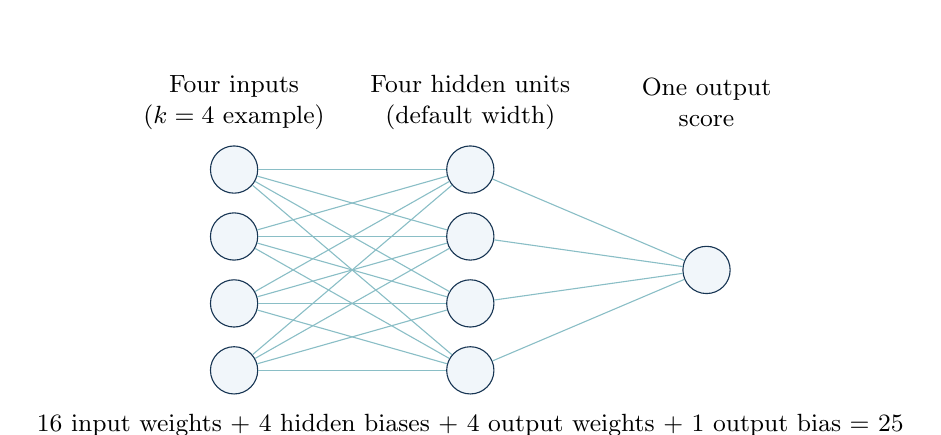
\begin{tikzpicture}[n/.style={circle,draw=navy,fill=pale,minimum size=6mm},
 line/.style={draw=teal!50},font=\small]
 \foreach \i in {1,...,4}{
   \node[n] (x\i) at (0,-0.85*\i) {};
   \node[n] (h\i) at (3,-0.85*\i) {};
 }
 \node[n] (o) at (6,-2.125) {};
 \foreach \i in {1,...,4}{
   \foreach \j in {1,...,4}{\draw[line] (x\i)--(h\j);}
   \draw[line] (h\i)--(o);
 }
 \node[align=center] at (0,0) {Four inputs\\($k=4$ example)};
 \node[align=center] at (3,0) {Four hidden units\\(default width)};
 \node[align=center] at (6,0) {One output\\score};
 \node[align=center] at (3,-4.1) {16 input weights + 4 hidden biases + 4 output weights + 1 output bias = 25};
\end{tikzpicture}
\caption{B at four input features. Lines represent learned connections;
biases are counted but not drawn. This is an architecture diagram, not a
trained network visualization.}
\end{figure}

\subsection{Why intentionally limit the model?}
A small model provides a useful reference for data scarcity and model size.
It is not automatically accurate, robust, or interpretable just because it is
small. A small capacity can constrain memorization, but may also prevent the
model from expressing a useful decision rule. Both possibilities are testable.

For hidden width $h$, the parameter count is
\begin{equation}
 P_B=kh+h+h+1=h(k+2)+1.
\end{equation}
At default $h=4$, this is 17, 25, or 33 for 2, 4, or 6 inputs. These are
weights and biases, not qubits. Matching this number to the number of trainable
quantum angles would still not guarantee equal expressiveness or compute cost.

B uses L-BFGS optimization and two candidate L2 regularization strengths,
$10^{-4}$ and $10^{-2}$. L2 regularization penalizes large weights. The
validation data select its strength; test examples do not. B's existing fit
does not use class weights, so imbalance treatment differs from A and D.

\subsection{What a weak or strong B result means}
If B performs well, the task may not require a large learned mapping on the
chosen features. If it performs poorly, possible explanations include too
little capacity, a poor representation, imbalance, or incomplete optimization.
One score cannot distinguish these explanations. Its output 0.8 also does not
establish an 80\% real-world probability of drone presence without calibration.

\section{Model C: testing additional neural capacity}
\label{sec:modelc}
\plain{C receives the same short description as B but has more intermediate
units and another layer. It can construct more combinations of those inputs.
It still cannot see information that was discarded before the input arrived.}

The two-hidden-layer network is
\begin{align}
 \mathbf{h}_1&=\operatorname{ReLU}(W_1\mathbf{x}+\mathbf{b}_1),\\
 \mathbf{h}_2&=\operatorname{ReLU}(W_2\mathbf{h}_1+\mathbf{b}_2),\\
 p_C&=\sigma(\mathbf{v}^{\mathsf T}\mathbf{h}_2+c).
\end{align}
The first layer combines input features. The second combines first-layer
responses. The implementation tries widths $(64,32)$ and $(128,64)$, each
with the same two regularization choices used for B.

At $k=4$, those networks contain 2,433 and 8,961 parameters. The first count
can be checked as $(4+1)64+(64+1)32+(32+1)1=2433$. The ``+1'' at each
stage accounts for the bias of each unit in the next layer.

\subsection{Why C is needed alongside B}
Comparing a quantum method only with a tiny neural model leaves an obvious
alternative explanation: perhaps the classical baseline was too small.
C helps test that explanation without changing the compact feature inputs.
It is a stronger capacity reference, not a promised performance ceiling.

A C-over-B improvement could reflect capacity, optimization, or selection
budget, since C has more candidates. Report those differences. If C memorizes
the training set but fails on validation, that does not justify choosing it
because it has more parameters. If B and C both fail, adding more hidden units
cannot necessarily repair information loss from averaging or PCA.

\subsection{Why not make C arbitrarily large?}
The research question concerns limited independent data. An unrestricted
architecture search would consume more computation and expose the validation
set to more decisions, making results harder to interpret. Two specified
architectures provide a bounded comparison. The maximum iteration count is
an optimization limit, not proof of convergence; inspect convergence warnings
and preserve all candidate validation scores.

\section{Model D: a small spectrogram CNN}
\label{sec:modeld}
\plain{D gets a time-frequency map instead of a short summary. It scans small
regions for learned patterns, combines those responses, and produces one
score. This tests whether information lost by the compact summary matters.}

Convolution shares a small filter across positions. This reduces the number
of separately learned coefficients relative to connecting every position
independently~\cite{convbook}. In this project the filters might respond to
bands or changing spectral patterns, but their actual behavior must be
inspected after training. Naming the task ``drone detection'' does not force
the network to learn rotor-specific cues.

\begin{center}
\small
\begin{tabularx}{\linewidth}{@{}lYr@{}}
\toprule
Stage & Meaning in this architecture & Parameters \\
\midrule
Conv $1\rightarrow16$ & Sixteen $3\times3$ filters, ReLU, then max pooling & 160 \\
Conv $16\rightarrow32$ & Combine local responses, ReLU, then max pooling & 4,640 \\
Conv $32\rightarrow64$ & Further learned local combinations and ReLU & 18,496 \\
Global average & One spatial mean per final feature map & 0 \\
Dense $64\rightarrow32$ & Combine map summaries, ReLU, dropout 0.2 & 2,080 \\
Dense $32\rightarrow1$ & Produce the final logit & 33 \\
\midrule
Total & Sigmoid converts the logit to an inference score & 25,409 \\
\bottomrule
\end{tabularx}
\end{center}
The numbers 16, 32, and 64 refer to learned feature maps, not microphones.
Each convolution has stride one and padding one. The first two $2\times2$
max-pooling stages reduce spatial resolution. Global averaging controls the
dense head size but discards exact locations in the final maps. The current
workspace implements that averaging as an explicit spatial mean.

\subsection{What training tries to improve}
\plain{Training is practice with a scorekeeper. After each guess, the
scorekeeper gives a penalty: small when the guess was right, large when the
model was confident and wrong. The model's numbers are nudged, again and again,
in the direction that makes the penalty smaller.}

The final raw output $a_i$ is a \emph{logit}. With label $y_i$, the weighted
binary cross-entropy objective is
\begin{equation}
 \mathcal L=-\frac{1}{B}\sum_{i=1}^{B}
 \left[w_+y_i\log\sigma(a_i)+(1-y_i)\log(1-\sigma(a_i))\right].
\end{equation}
Here $B$ is the mini-batch size, not Model B. The factor
$w_+=N_0/N_1$ gives positive examples a weight based on training-window
class counts. A confident wrong prediction incurs a large loss. The code uses
a numerically stable logit-based implementation rather than directly taking
logs of rounded probabilities.

Adam updates the parameters~\cite{adam}; the defaults are learning rate
$10^{-3}$, weight decay $10^{-4}$, 30 epochs, and batch size 32.
An epoch is one pass through the training examples. Dropout suppresses some
dense activations during training, while inference uses the full
network~\cite{dropout}. The best validation checkpoint is retained. Running
all requested epochs and selecting the best checkpoint is different from
stopping early after a fixed patience period.

\subsection{Why D belongs, and why it is a different comparison}
D tests a representation question as well as a classifier question. If it
outperforms A--C, the gain could arise from retained temporal structure,
optimization, or architecture. It does not establish that convolution alone
caused the difference. Conversely, a small independent training set may be
insufficient for D despite its richer input.

Possible failures include sensitivity to microphone changes, learning
background or session cues, and losing short events when scores are averaged
over a long recording. D is therefore valuable as an application-oriented
reference, while the compact-feature quantum comparison should identify it
separately. Its parameter count is fixed by the architecture, but its compute
and memory costs still depend on window duration and batch size.

\section{Experimental design: making the comparison answer the question}
\label{sec:design}
\subsection{Reproduction and strict scarcity are different studies}
\plain{Suppose a student is told which facts matter by someone who studied
301 flashcards, and then practises with only 24 of them. The student has still
been helped by all 301. If the question is ``what can be learned from 24?'',
every step has to use only those 24.}

The previously reviewed teammate protocol uses 24, 80, and 98 independent
recording units for the initial training, validation, and test comparison.
However, its saved selected-feature ranking was developed using 301 labeled
training recordings before the smaller classifier subset was chosen.

There are two valid but different questions. \emph{Reproduction} asks what
happens when we preserve that original development procedure and its exact
features. \emph{Strict scarcity} asks what can be learned when the permitted
training-label budget really is limited to the selected subset. For strict
scarcity, supervised feature ranking must also stay inside that subset.
Fit scalers there too, and disclose any additional noise/development data.

The validation-label budget must also be reported. A method fitted on 24
training recordings but selected with 80 labeled validation recordings has
not consumed only 24 labels in its entire development process. Both counts
matter, especially when comparing learning under label scarcity.

\subsection{Agree on what constitutes one prediction}
\plain{There are two ways to judge a long recording. One is to blend all of
its pieces together and judge the blend once. The other is to judge every
piece and average the verdicts. The two can disagree, so both teams must use
the same one.}

The original pipeline scores windows and averages scores. The teammate's
quantum comparison averages features per source recording before classification.
For a nonlinear model, these are generally different:
\begin{equation}
 f\!\left(\frac{1}{m}\sum_{j=1}^m\mathbf{x}_j\right)
 \neq \frac{1}{m}\sum_{j=1}^m f(\mathbf{x}_j).
\end{equation}
The left side summarizes the evidence before making a decision. The right
side makes multiple decisions and summarizes the scores. Neither should be
silently substituted for the other. Preserve source-group IDs across files,
match the A--C feature-aggregation order to the intended quantum experiment,
and document D's window-score aggregation separately.

\subsection{Pre-specified comparison procedure}
\begin{enumerate}
 \item Freeze the dataset versions, label definitions, source-group splits,
 and recording-level evaluation IDs. Validate any imported IDs against the
 original tables rather than merely matching their counts.
 \item Choose reproduction or strict scarcity. Freeze window duration,
 feature representation, aggregation, SNR conditions, noise donors, and
 silence policy. Save every exclusion with a reason.
 \item Draw balanced nested training subsets at feasible sizes such as
 24, 50, and 70 recordings. A smaller subset should belong to the same seed's
 larger subset. Each model receives the same subset for that seed.
 \item Fit preprocessing on the permitted training data. Choose candidate
 models using the agreed validation rule. Keep optimizer settings and search
 budgets in the experiment record.
 \item Freeze configurations and evaluate the aligned test recordings at all
 requested SNRs. Save individual scores, not only summary metrics.
 \item Repeat using a declared seed list. Report means and variability, as
 well as paired per-recording comparisons. Rerun quantum models if the
 preprocessing or data budget changes.
\end{enumerate}
The baseline defaults to validation balanced accuracy. The matched tabular
runner can select by F1 with balanced accuracy and drone recall as tie-breakers.
D currently selects checkpoints using balanced accuracy. That difference
must be retained in the report or harmonized before claiming identical
selection rules across all models.

\subsection{Ablations: changing one choice at a time}
An \emph{ablation} isolates an experimental choice. Useful planned comparisons
include clean training versus noisy augmentation, one- versus three-second
windows, compact PCA features versus the selected-feature representation,
and small versus larger neural capacity. Keep other settings fixed whenever
the comparison permits. D-versus-C cannot isolate a single cause because both
their inputs and their architectures change.

\section{Evaluation: what does ``good'' mean?}
\label{sec:metrics}
\plain{A detector can be wrong in two different ways. It can cry ``drone''
when there is none (a false alarm), or stay quiet when a drone is there (a
miss). One score cannot describe both mistakes, so we count them separately.}

An alert can be right or wrong, and the absence of an alert can also be right
or wrong. The resulting confusion matrix contains four counts:
\begin{center}
\begin{tabular}{@{}lcc@{}}
\toprule
 & Predict drone & Predict non-drone \\
\midrule
Actual drone & True positive (TP) & False negative (FN) \\
Actual non-drone & False positive (FP) & True negative (TN) \\
\bottomrule
\end{tabular}
\end{center}
Recall asks how many actual drones are found. Precision asks how many drone
alerts are correct. Specificity asks how many negatives are correctly rejected:
\begin{align}
 \mathrm{Recall}&=\frac{TP}{TP+FN},&
 \mathrm{Precision}&=\frac{TP}{TP+FP},\\
 \mathrm{Specificity}&=\frac{TN}{TN+FP},&
 \mathrm{Accuracy}&=\frac{TP+TN}{TP+FN+FP+TN}.
\end{align}
Balanced accuracy weights the two class recalls equally. F1 combines precision
and recall:
\begin{equation}
 \mathrm{BA}=\tfrac12(\mathrm{Recall}+\mathrm{Specificity}),\qquad
 F_1=\frac{2TP}{2TP+FP+FN}.
\end{equation}
ROC-AUC evaluates score ranking across thresholds; it needs both classes and
does not replace assessment at the chosen operating threshold. Neither an
SVM decision value nor an uncalibrated sigmoid score should be presented as
an established probability of safety or drone presence.

\subsection{Worked example: why accuracy alone can mislead}
\textbf{Instructional example only---not project results.} Suppose a test set
contains 10 drone and 90 non-drone recordings. A system that always predicts
non-drone is 90\% accurate, yet detects no drones. Its recall is zero,
balanced accuracy is 50\%, and F1 is zero under the project's zero-division policy.

Now consider a hypothetical detector with TP=8, FN=2, FP=9, and TN=81:
\begin{center}
\begin{tabular}{@{}ll@{}}
\toprule
Metric & Calculation \\
\midrule
Accuracy & $(8+81)/100=89\%$ \\
Recall & $8/10=80\%$ \\
Precision & $8/17\approx47.1\%$ \\
Specificity & $81/90=90\%$ \\
Balanced accuracy & $(80\%+90\%)/2=85\%$ \\
F1 & $16/(16+9+2)\approx59.3\%$ \\
\bottomrule
\end{tabular}
\end{center}
Its accuracy is slightly lower than the useless all-negative detector, but it
finds eight of the ten drones. Whether nine false alarms are acceptable is
an application requirement; a single headline metric cannot decide that.

\subsection{Uncertainty and the unit of evidence}
Changing the seed can change a training subset or initialization. Report that
variability rather than just the most favorable seed. Repeating seeds on the
same test recordings does not create independent new test data. For proposed
bootstrap confidence intervals, resample independent source groups rather
than individual correlated windows, and retain paired model predictions.
The evaluated recording count and class balance must accompany the metrics.

\section{Computation, reproducibility, and hardware}
\label{sec:hardware}
\plain{A graphics card (GPU) is a faster calculator for one kind of
arithmetic. It can make Model D finish sooner. It does not make any model's
answers more correct, and it cannot repair a badly designed experiment.}

A--C use CPU-based scikit-learn implementations. A GPU does not automatically
accelerate those estimators. D uses PyTorch and supports \code{auto},
\code{cpu}, and \code{cuda} device modes. Automatic mode tests visible CUDA
devices with a small operation, chooses a usable one, and falls back to CPU
when none works. A forced CUDA request fails when no usable GPU is found.

An A100, L40S, or newer compatible NVIDIA GPU can execute the CNN when the
driver and PyTorch build support it. The code does not require a particular
GPU model name and does not distribute training over multiple GPUs. A
CPU-only PyTorch installation remains CPU-only even on a machine containing
an NVIDIA GPU. The automatic non-CUDA fallback is CPU, not an automatic
choice of Apple MPS or another vendor's backend.

The model and mini-batches move to the selected device, and inference scores
return to CPU for reporting. Checkpoints store CPU tensors for portability.
Seeds and deterministic settings help reproduction, but exact agreement across
hardware and software versions is not guaranteed~\cite{repro}. A faster device
changes execution time; it does not turn an invalid split into a valid experiment.

\textbf{A useful workload calculation.} If 24 recordings each last ten minutes,
three-second segmentation produces approximately
$24\times600/3=4800$ windows before exclusions. Adding four noisy copies
would make five versions of each window, or approximately 24,000 examples.
These are illustrative counts, not an inventory of the current dataset.
They explain why a recording count alone is insufficient to predict training time.

Audio loading and feature extraction remain important CPU costs. Measure
preparation, fitting, and inference separately as well as end-to-end time.
Caching unchanged features across runs can reduce repeated work. A CUDA
availability probe is not a training-memory reservation or a completed
accelerator benchmark.

\section{Results status and proposed reporting format}
\label{sec:status}
\textbf{There are no new experimental results in this paper.} No model was
trained to write it. The architecture counts are derived from the code, the
worked confusion matrix is hypothetical, and the workflow diagrams are
schematic. Earlier software checks should not be interpreted as evidence of
real-world detection quality or as validation of every later code change.

A completed study should report at least the following fields for each
configuration; the table deliberately contains no fabricated scores:
\begin{center}
\begin{tabularx}{\linewidth}{@{}lY@{}}
\toprule
Field & What to record \\
\midrule
Protocol & Reproduction or strict scarcity; feature mode and aggregation \\
Data budget & Training, validation, and test source counts; per-class counts \\
Model settings & A/B/C/D, feature width, architecture, regularization, optimizer \\
Noise & Train/test SNR, donor IDs, exclusions, actual evaluated IDs \\
Selection & Validation metric, candidate budget, selected candidate/checkpoint \\
Performance & Accuracy, balanced accuracy, precision, recall, F1, specificity, AUC \\
Uncertainty & Declared seeds, per-seed results, paired recording-level analysis \\
Resources & Parameters or support vectors, preprocessing/fit/inference time \\
Provenance & Dataset release, code fingerprint, versions, device, saved predictions \\
\bottomrule
\end{tabularx}
\end{center}
Imported teammate results can be used for reproduction only after verifying
that sample IDs, feature values, preprocessing, and aggregation agree. A
corrected protocol requires new matched results, including quantum reruns
where relevant. An empty result cell is preferable to a plausible invented one.

\section{Discussion and threats to validity}
\plain{A ``threat to validity'' is a way the experiment could give a pleasing
answer for the wrong reason. Listing these in advance is how a study earns
trust: it tells the reader what the results will and will not show.}

\subsection{Dataset identity can become a shortcut}
If nearly all positives come from one microphone or dataset and nearly all
negatives from another, a classifier can exploit collection differences.
Grouping prevents direct source overlap but does not remove all domain
confounding. Examine performance by dataset and acquisition condition, and
prefer negative recordings collected under comparable conditions when available.

\subsection{Synthetic mixtures are a controlled test, not the whole world}
Adding one background waveform at a specified SNR isolates a useful stress
condition. It does not reproduce every effect of real outdoor propagation,
microphone saturation, changing distance, or multiple moving sources.
``Robust at 0 dB'' must refer to the tested mixture procedure and data, not all
possible environments with that label.

\subsection{Labels and aggregation define the task}
A long recording labeled drone may contain periods with no audible drone.
Assigning its label to every window creates weak window labels. Averaging
scores may also suppress a short event within mostly negative audio. Decide
whether the target is recording presence, window presence, or event timing,
and collect labels suitable for that target. These are different detection tasks.

\subsection{Capacity and information budgets are not interchangeable}
B's small parameter count does not prove a fair match to a quantum circuit.
C's greater capacity does not guarantee better generalization. D receives
more detailed inputs. A's support-vector count measures something different
from a neural weight count. A defensible claim states exactly which resource
and representation constraints were matched.

\subsection{The implementation is not yet deployment evidence}
The code can produce labels and a frontend can display them, but deployment
would require operating-threshold decisions, calibration checks, latency and
memory measurements, monitoring of changing conditions, and a defined
response to uncertain inputs. False alarms per unit time would require an
appropriate continuous-recording evaluation; clip-level specificity alone is
not that quantity.

\section{Conclusion}
A meaningful acoustic drone study needs more than a classifier with a high
score. It needs a precise label definition, independent sources, a documented
feature representation, controlled noise conditions, and model selection that
does not use the test set. A tests a conventional nonlinear kernel, B tests a
small neural mapping, C tests additional capacity on the same compact inputs,
and D tests a richer time-frequency representation.

The proposed study can reveal whether limitations come from information loss,
model capacity, noise, or transfer across recording conditions, although
additional controlled experiments may be needed to separate those causes.
It can also provide a credible classical comparison for quantum experiments.
Which model performs best, and whether any quantum difference survives the
matched protocol, remain empirical questions.

\appendix
\section{Glossary for a first-time reader}
\label{sec:glossary}
\begin{longtable}{@{}p{3.1cm}p{13.0cm}@{}}
\toprule
Term & Meaning in this study \\
\midrule
\endhead
Acoustic & Related to sound measured by a microphone. \\
Augmentation & Additional training versions, such as noisy copies, derived from existing examples. \\
Baseline & A reference method used to judge another method under stated conditions. \\
Batch & A group of examples processed together during a neural-network update. \\
Calibration & Whether predicted probability values agree with observed frequencies on appropriate held-out data. \\
Confuser & A non-drone sound that may resemble a drone in the chosen representation. \\
CUDA & NVIDIA's GPU computing platform used by a compatible PyTorch installation. \\
Epoch & One pass through the training examples. \\
Feature & A numerical description calculated from audio. \\
Generalization & Performance on genuinely new examples drawn from the intended task. \\
Hyperparameter & A setting selected outside a model's parameter-fitting procedure. \\
Inference & Applying fixed model parameters to new inputs. \\
Kernel & A function expressing similarity between two inputs. \\
Leakage & Information crossing an experimental boundary in a way that invalidates the intended evaluation. \\
Logit & A neural network's raw binary output before the sigmoid. \\
MFCC & Mel-frequency cepstral coefficient; a numerical representation derived from a log-mel spectrum. \\
Parameter & A fitted weight, bias, or other learned model quantity. \\
PCA & Principal component analysis; a training-fitted linear reduction of feature dimensions. \\
Regularization & A constraint or penalty intended to control aspects of model fitting. \\
Seed & A value controlling a pseudo-random sequence for reproducible draws or initialization. \\
SNR & Signal-to-noise ratio; here, the original target's power relative to added noise power. \\
Source group & Related audio that must remain together when splitting independent examples. \\
Spectrogram & A matrix describing frequency content over time. \\
Threshold & The score above which a positive prediction is made. \\
Window & A short segment of audio used as an input unit. \\
\bottomrule
\end{longtable}

\section{Implementation correspondence and provenance}
This paper is a conceptual explanation with implementation details checked
against the workspace on October 7, 2026. Its own file fingerprints are in
\code{classical_approach_beginner_sources.json}. It is separate from the
earlier technical report, whose explicit baseline snapshot remains documented
in \code{classical_approach_sources.json}. Both describe the same project
source~\cite{source}.

The current workspace contains \code{data.py} for manifests and audio,
\code{models.py} for tabular fitting and metrics, \code{cnn.py} for Model D
and device handling, \code{cli.py} for waveform experiments,
\code{matched.py} for selected-feature reproduction/strict protocols,
\code{dhanya.py} for imported assets, and artifact/subset utilities.
Recent interfaces include configurable window duration, silent-window policy,
recording-level outputs, and training-size/seed sweeps. Their presence in
source is not presented as a newly validated benchmark in this document.

The matched selected-feature runner covers A--C. D needs corresponding audio
and remains a richer-input reference. Imported assets must be available and
validated before a matched experiment is run. No data were invented to fill
missing manifests, and no training command was executed to produce this paper.

% Bibliography is embedded below so this file remains standalone.
\begin{thebibliography}{99}
\bibitem{svmoriginal}
C. Cortes and V. Vapnik. ``Support-vector networks.''
\emph{Machine Learning}, 20, pp. 273--297, 1995.
\href{https://doi.org/10.1007/BF00994018}{doi:10.1007/BF00994018}.

\bibitem{svc}
scikit-learn developers. \emph{SVC API reference}.
\href{https://scikit-learn.org/stable/modules/generated/sklearn.svm.SVC.html}{Official support vector classifier documentation}.

\bibitem{mlp}
scikit-learn developers. \emph{MLPClassifier API reference}.
\href{https://scikit-learn.org/stable/modules/generated/sklearn.neural_network.MLPClassifier.html}{Official multilayer perceptron documentation}.

\bibitem{convbook}
I. Goodfellow, Y. Bengio, and A. Courville. \emph{Deep Learning}.
MIT Press, 2016, Chapter 9.
\href{https://www.deeplearningbook.org/contents/convnets.html}{Convolutional Networks}.

\bibitem{dropout}
N. Srivastava, G. Hinton, A. Krizhevsky, I. Sutskever, and R. Salakhutdinov.
``Dropout: A Simple Way to Prevent Neural Networks from Overfitting.''
\emph{Journal of Machine Learning Research}, 15(56), pp. 1929--1958, 2014.
\href{https://www.jmlr.org/papers/v15/srivastava14a.html}{Original article}.

\bibitem{adam}
D. P. Kingma and J. Ba. ``Adam: A Method for Stochastic Optimization.''
2014. \href{https://arxiv.org/abs/1412.6980}{arXiv:1412.6980}.

\bibitem{ddl}
S. Safavi, M. A. Safavi, B. Cook, and W. Wang.
\emph{DDL: Dataset and Baseline Methods for Drone Detection and Localization
Using Sound}. Zenodo, version v1, 2023.
\href{https://doi.org/10.5281/zenodo.6459183}{doi:10.5281/zenodo.6459183}.
\href{https://zenodo.org/records/6459183}{Dataset and archive download page}.

\bibitem{esc50}
K. J. Piczak. ``ESC: Dataset for Environmental Sound Classification.''
\emph{Proceedings of the 23rd ACM International Conference on Multimedia},
pp. 1015--1018, 2015.
\href{https://doi.org/10.1145/2733373.2806390}{doi:10.1145/2733373.2806390}.
\href{https://github.com/karolpiczak/ESC-50}{Official ESC-50 dataset repository}.

\bibitem{urbansound}
J. Salamon, C. Jacoby, and J. P. Bello.
``A Dataset and Taxonomy for Urban Sound Research.''
\emph{Proceedings of the 22nd ACM International Conference on Multimedia},
2014.
\href{https://urbansounddataset.weebly.com/urbansound8k.html}{Official UrbanSound8K dataset and metadata description}.
\href{https://urbansounddataset.weebly.com/}{Publication and attribution page}.

\bibitem{nasa}
National Aeronautics and Space Administration (NASA).
\emph{Small UAS Flyover Acoustics Data}. NASA Open Data Portal.
\href{https://data.nasa.gov/dataset/small-uas-flyover-acoustics-data}{Official dataset, archive, and data-description links}.
Accessed October 7, 2026.

\bibitem{svanstrom}
F. Svanstr\"om.
\emph{DroneDetectionThesis/Drone-detection-dataset: First release}.
Zenodo, version v1.0.0.
\href{https://doi.org/10.5281/zenodo.5500576}{doi:10.5281/zenodo.5500576}.
\href{https://zenodo.org/records/5500576}{Dataset release page}.

\bibitem{ituaris}
\.I. M. Muhac{\i}ro{\u{g}}lu and T. Akg\"ul.
\emph{ITU ARIS Lab. Acoustic Drone Dataset}.
Zenodo, version 1.0.0, 2026.
\href{https://doi.org/10.5281/zenodo.22682339}{doi:10.5281/zenodo.22682339}.
\href{https://huggingface.co/datasets/imm61/itu-aris-lab-acoustic-drone-dataset}{Dataset card, group mappings, and split documentation}.

\bibitem{librosa}
librosa developers. \emph{librosa.feature.mfcc}, version 0.11.0 documentation.
\href{https://librosa.org/doc/0.11.0/generated/librosa.feature.mfcc.html}{Official MFCC API reference}.

\bibitem{repro}
PyTorch contributors. \emph{Reproducibility}.
\href{https://docs.pytorch.org/docs/stable/notes/randomness.html}{Official reproducibility notes}.

\bibitem{source}
QubitSky Project. \emph{Classical implementation source}.
\code{qsky_classical/} package, \code{BENCHMARK_PROTOCOL.md},
\code{QubitSky_DATASETS.md}, and \code{DATASET_SETUP.md}. October 7, 2026.
See \code{classical_approach_beginner_sources.json} for SHA-256 fingerprints.
\end{thebibliography}
\end{document}
